\documentclass{aip-cp}

\usepackage[numbers]{natbib}
\usepackage{rotating}
\usepackage{graphicx}

%% ��� �������� ������ ���������������� �����!
%\usepackage{inputenc}
%\usepackage[T2A,T1]{fontenc}
%\usepackage[english,russian]{babel}
%\usepackage{cmap}
%%


% Document starts
\begin{document}

% Title portion
\title{Using Machine Learning for Separation of Parameters in High-Dimensional Global Optimization Problems}

\author[aff1]{Konstantin Barkalov\corref{cor1}}
\author[aff1]{Marina Usova}

\affil[aff1]{Lobachevsky State University of Nizhny Novgorod, Nizhny Novgorod, Russia}
\corresp[cor1]{Corresponding author: konstantin.barkalov@itmm.unn.ru}

\maketitle

\begin{abstract}
This paper examines the findings from research into an approach to solving optimization problems, in which the dependencies on diverse groups of parameters are of a different nature.
A scheme has been proposed for choosing the problem parameters, which have a local effect on the objective function.
It allows solving essentially  multidimensional problems using the nested optimization scheme.
In this case,  different optimization algorithms are used at differing nesting levels.
The proposed approach has demonstrated its efficiency in solving several series of test problems.

\end{abstract}

% Head 1
\section{INTRODUCTION}

At present, global optimization methods are applied to solving a variety of problems arising in various fields of science and technology (see \cite{Pinter2006}). 
For example, the evaluation of the model parameters from the experimental data is a traditional field of application of the global optimization methods.
Such applications include chemical kinetics problems (see \cite{Gubaydullin2021}).
In the problems of this kind, it is necessary to perform a search for the values of unknown model parameters, at which the modeling results are closest to those obtained experimentally.

The number of parameters to be evaluated in this way can be tens and hundreds for chemical kinetics problems.
The use of deterministic global optimization methods for solving the problems of such a dimensionality is very limited because of very large computation costs of covering the search domain by trial points.
This holds even in the case when efficient algorithms (for example, \cite{Paulavicius2011,Evtushenko2009,Jones2009,Paulavicius2020,Sergeyev2021}) are used to construct the essentially nonuniform coverages. 

Numerous inverse problems are characterized by different dependencies on varying groups of parameters. 
For example, the dependence on one group of parameters may be close to the linear one whereas the dependence on another group of parameters may have a complex multiextremal nature.
In this case, the problem can be solved using the recursive optimization scheme. 
A multiextremal subproblem will be solved at the upper nesting level with the use of complex global optimization algorithms.
Unimodal subproblems (each corresponding to a fixed set of the values of the first part of parameters) will be solved at the lower nesting level.
To solve such problems, one can apply local optimization methods having a fast convergence. 

As a rule, one cannot subdivide the parameters into groups with different nature of the objective function behavior in advance since the objective function in applied problems is usually defined as a black box. 
To date, the development of an algorithm for the minimization of essentially multiextremal functions taking into account the different nature of the dependence of the objective function on various groups of parameters is quite relevant. 
In the present work, a special method for such a separation based on the analysis of the regression model of the function with respect to each variable separately has been proposed.
To confirm the efficiency of the scheme proposed, a representative set of test problems has been solved.

\section{OPTIMIZATION ALGORITHMS AND DIMENSIONALITY REDUCTION}

The paper considers an optimization problem of the form 
\begin{eqnarray}\label{main_problem}
& \varphi(y^\ast)=\min{\left\{\varphi(y): y\in D\right\}}, \nonumber \\
& D=\left\{y\in R^N: a_i\leq y_i \leq b_i, 1\leq i \leq N\right\}. \nonumber
\end{eqnarray}

Let us assume the function $\varphi(y)$ to be a multiextremal one and to satisfy the Lipschitz condition
\[
\left|\varphi(y')-\varphi(y'')\right|\leq L\left\|y'-y''\right\|,\; y',y'' \in D,\; 0<L<\infty,
\]
with the constant $L$ unknown {\em a priori}.
At the same time, let us assume the dependence of the objective function on $N_1$ parameters to be multiextremal while the dependence on the remaining $N_2 = N - N_1$ parameters is close to the linear or quadratic one.
At the same time, the subdivision of the parameters is unknown. 
In the present work, an approach to the separation of the problem parameters into the two specified groups is proposed.
The details of the method are described in the next section. 

Taking into account such a specific feature of the problem can essentially reduce the computation costs of the search for the optimum. 
Indeed, according to well known nested optimization scheme \cite{Grishagin2001,Grishagin2015}, the initial problem can be solved in the following way:
\begin{equation}\label{global_problem}
\varphi(y^*) = \min_{y\in D} \varphi (y) = \min_{y^1\in D_1} f(y^1), \; D_1=\left\{y\in R^{N_1}: 
a_i\leq y_i \leq b_i, \; 1\leq i \leq N_1\right\},
\end{equation}
where 
\begin{equation}\label{local_problem}
f(y^1) = \min_{ y^2 \in D_2} \varphi(y^1,y^2), \; D_2=\left\{y\in R^{N_2}: a_i\leq y_i \leq b_i, \; 
N_1+1\leq i \leq N\right\}.
\end{equation}

According to (\ref{global_problem}), the computation of a single value of the function $f(y^1)$
%(this process will be called {\em a search trial})
implies solving the unimodal problem (\ref{local_problem}), which can be performed by one of local optimization methods.
The efficiency of local optimization methods makes it possible to solve the subproblems (\ref{local_problem}) with an accuracy essentially exceeding the accuracy of global optimization methods.
Accordingly, we can consider the problem (\ref{global_problem}) as a global optimization problem where the process of computing an objective function value is a 
time-consuming operation. 

In the present study, we used the global search algorithm combined with the dimensionality reduction scheme based on Peano curves \cite{Sergeyev2013,Lera2015,Lera2021} to solve the global optimization problem (\ref{global_problem}). 
This algorithm was demonstrated to be a powerful tool for solving complex multiextremal problems (see \cite{Kvasov2013,Gillard2016,Kalyulin2017,Cavoretto2021}).
To solve the local problem (\ref{local_problem}), we used the Hooke-Jeeves (pattern search) method (see, e.g., \cite{Kelley}). 
Unlike the BFGS-type methods (see, e.g., \cite{Nocedal}), this algorithm does not require computing the gradient and works well under the conditions of computational errors in the function values, which is typical in solving applied problems.

\section{SEPARATION OF THE PROBLEM PARAMETERS}

To divide the problem parameters into the local and global ones, we propose the following sequence of operations.

Step 1. Fix the reference point $\overline{y} = (\overline{y}_1, \overline{y}_2,...,\overline{y}_N)$ for the objective function $\varphi(y)$. The choice of the point is performed by one of the following methods:
\begin{itemize}
\item the point is fixed according to the physical meaning of the applied problem being solved;
\item use the solution found by the local method (e.g. the  Hooke-Jeeves method) in $K$ iterations as the reference point;
\item use the solution found by the global method (e.g. the global search algorithm) in $K$ iterations as the reference point.
\end{itemize}

Step 2. For all components $y_i, \; 1\leq i \leq N$, investigate the locality:
\begin{enumerate}
\item[2.1] compute $P+1$ values of the objective function $\varphi(y)$ at the points $z_i^j = (\overline{y}_1,...,\overline{y}_{i-1},y_i^j,\overline{y}_{i+1},...,\overline{y}_N)$, where \mbox{$y_i^j = a_i + jh$},  $h=(b_i-a_i)/P, \; 0\leq j \leq P$;
\item[2.2] form a set $Q$ comprising $P+1$ pairs of the kind $\left\{y_i^j, \varphi(z_i^j)\right\} $ 
\item[2.3] construct a regression model of a given power $deg$ based on the data from $Q$;
\item[2.4] compute the coefficient of determination $R^2$ and perform the classification of the $i^{\rm th}$ variable:
\begin{itemize}
\item if $R^2$ is greater than a predefined threshold $T$, then add the variable to the set of the local variables;
\item else add the variable to the set of global variables.
\end{itemize}
\end{enumerate}

Step 3. If the local variables are found, then continue solving the problem using the nested optimization scheme; the global search algorithm will be used at the upper level while the local optimization method will be used at the lower one. Otherwise, run the global search algorithm, assuming all variables are global.

The regression is based on the least squares method (LSM).
The quality of the model constructed was evaluated at Step 2, Item 4 using the adjusted coefficient of determination $R^2_a$.
This coefficient characterizes the similarity of the regression model constructed to the objective function in the fixed section.
The value of $R^2_a$, as a rule, falls between 0 and 1.
A result close to 1 shows the accuracy of the model to be high.

The values of $K$, $deg$, and $T$ are the parameters of the method and are set by the researcher according to the properties of the problem being solved.
The algorithm makes it possible to use the power of the regression polynomial $deg = 1$ or $deg = 2$, which permits the construction of a model based on either linear or quadratic regression, respectively.

\section{NUMERICAL EXPERIMENTS}

In the first set of the test problems (we will denote it as Gr-L), we used 100 20-dimensional combined-type problems: a local subproblem of the dimensionality $N_2 = 18$ and a global subproblem of the dimensionality $N_1=2$.
The 18-dimensional subproblems comprising the combinations of nearly linear functions were used as the local component:
\begin{equation}\label{X2_problem}
\varphi_j^{loc}(y) = \sum_{i=1}^{18} \left(M_{ij} y_i + L_{ij} y_i^2\right), \; -2.2 \leq y_i \leq 1.8,
\end{equation}
where the parameters $0.5 \leq |M_{ij}| \leq 1$ and $0.01 \leq L_{ij} \leq 0.3$  were randomly uniformly distributed within the respective intervals.
The multiextremal functions proposed by Grishagin (see, for example, \cite{Grishagin1994}) were used as the global components of the problems $\varphi_j^{glob}(y)$. 
The objective function $\varphi(y)$ comprised a linear combination of these subproblems, i.e. $\varphi_j(y) = \alpha \varphi_j^{glob}(y) + \beta \varphi_j^{loc}(y)$. The sequence of parameters in each problem was selected randomly. 
Level lines of a multiextremal subproblem and a two-dimensional section of a local subproblem are shown in Figure \ref{fig}.

\begin{figure}
\begin{minipage}{0.27\linewidth}
\center{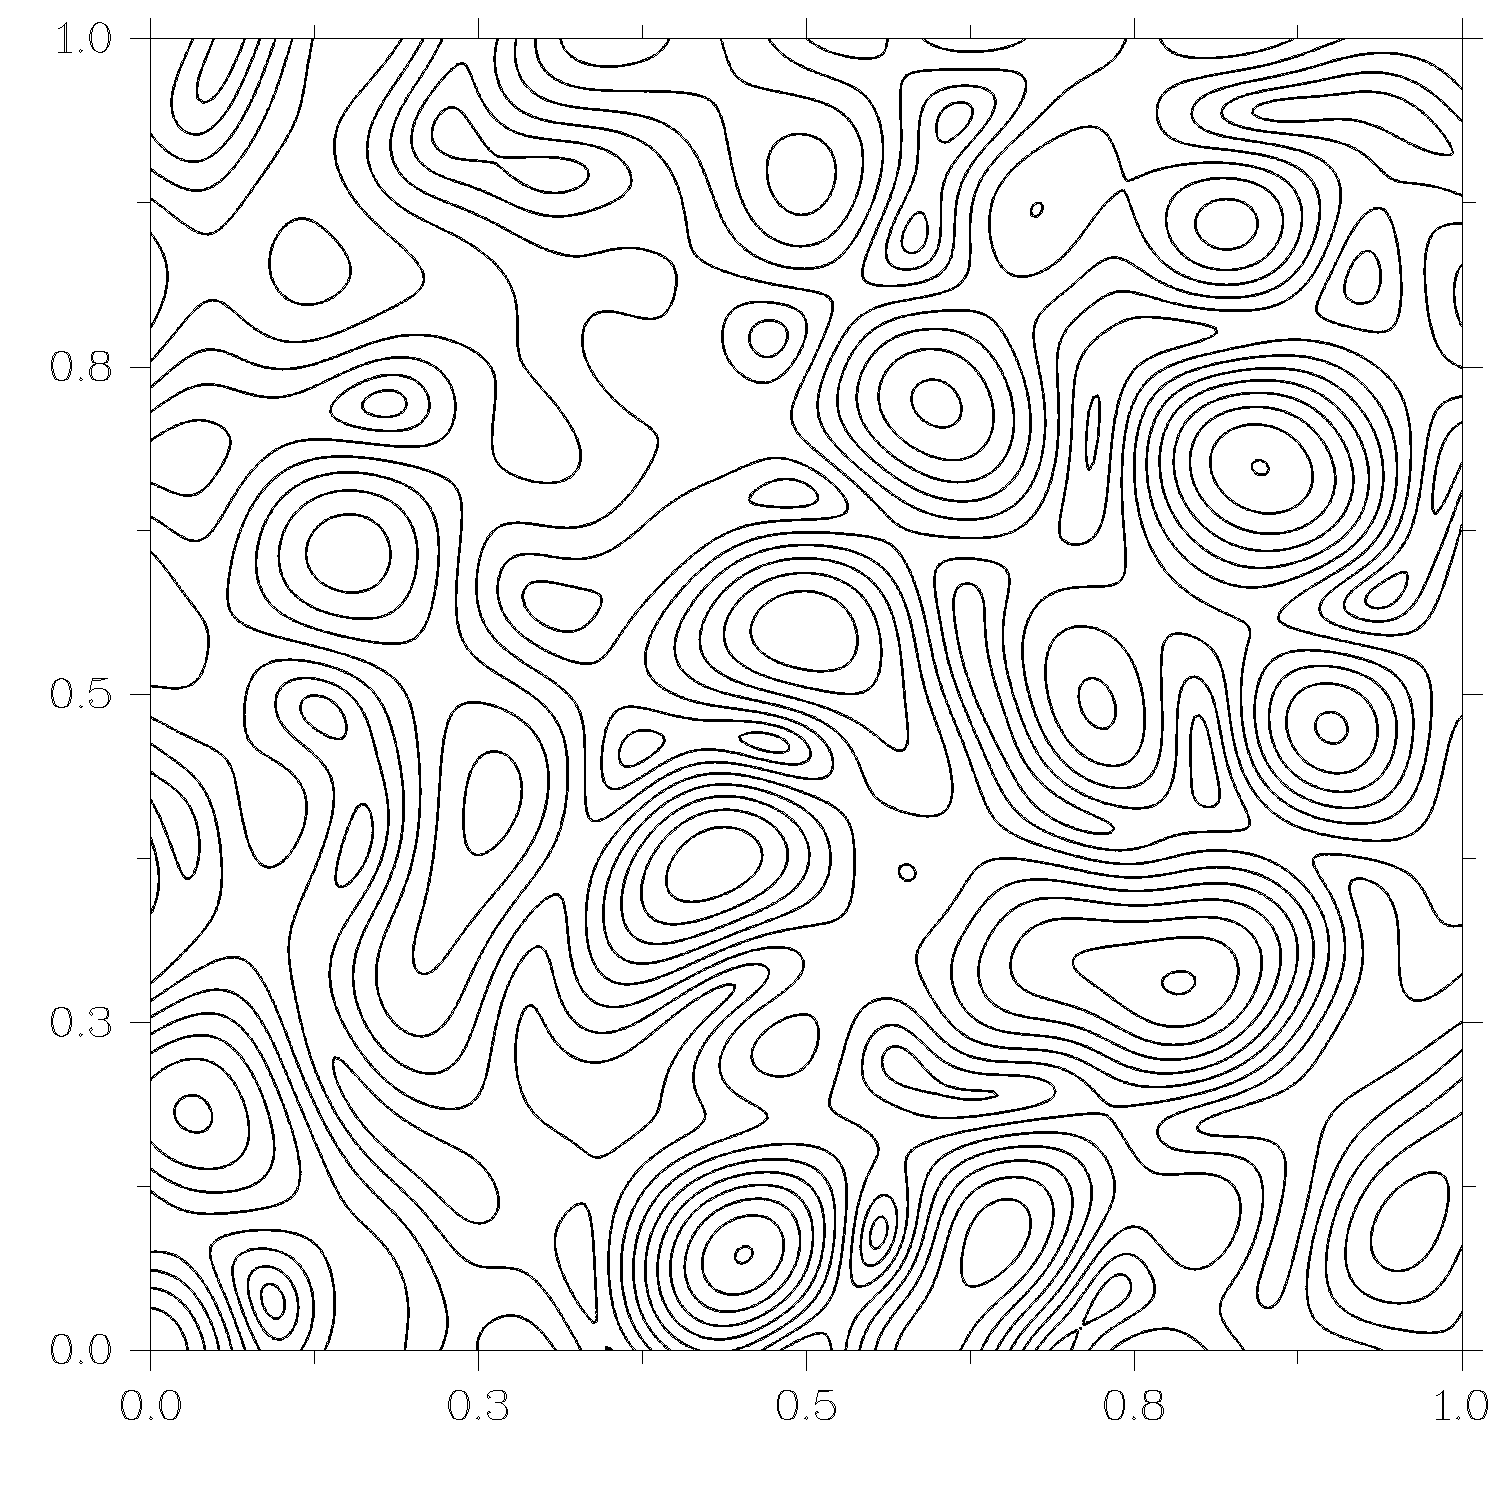
\includegraphics[width=1.0\linewidth]{fig1a.png}}
\end{minipage}

\;\;\;\;\;\;\;\;\;\;\;\;\;\;\;\;

\begin{minipage}{0.27\linewidth}
\center{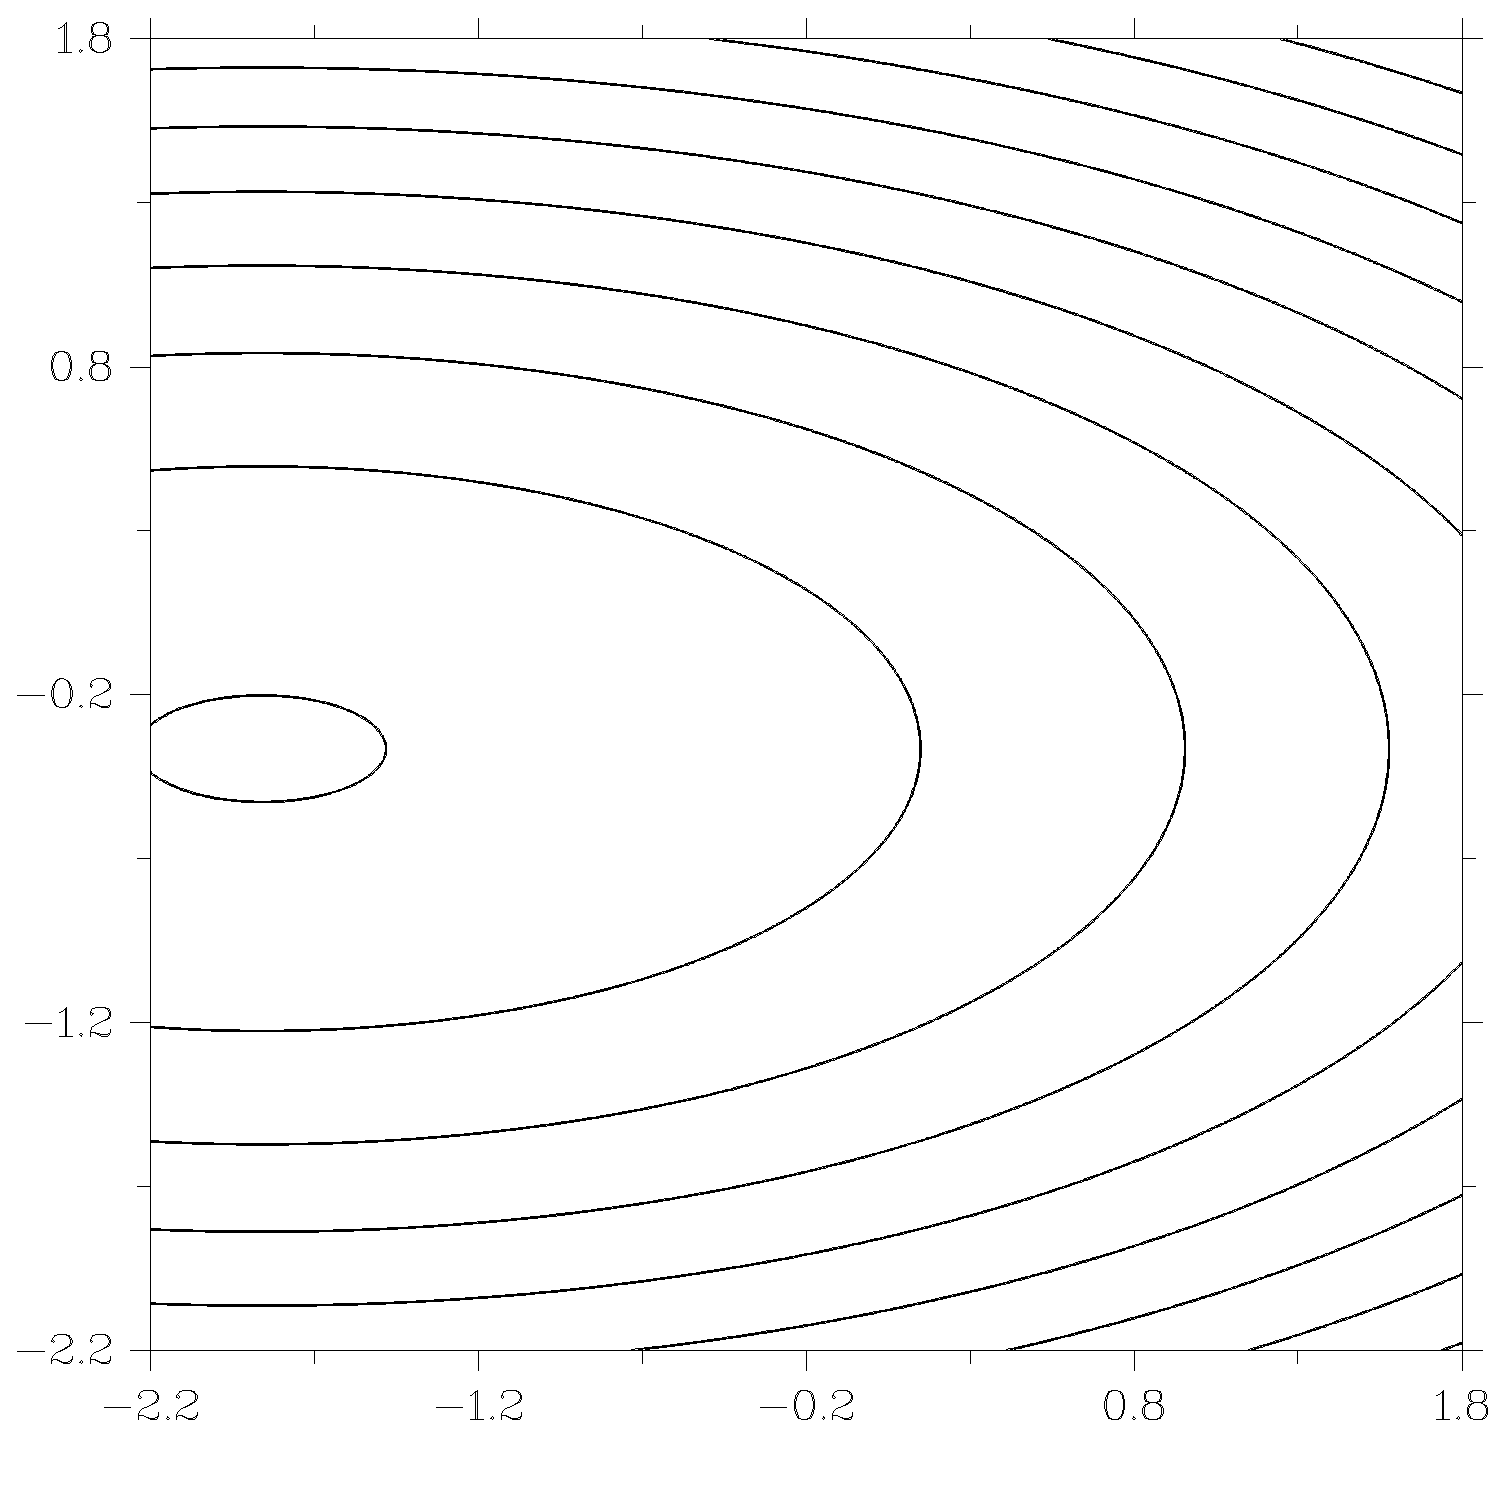
\includegraphics[width=1.0\linewidth]{fig1b.png}}
\end{minipage}
\caption{Level lines of a multiextremal subproblem and a two-dimensional section of a local subproblem.}
\label{fig}
\end{figure}


In the second set of problems (hereafter called Gr-LQ), the parameters $M_{ij}$ and $L_{ij}$ of the local subproblem (\ref{X2_problem}) were organized so that in 60\% of the cases the variable had an insufficient quadratic part, in 30\% of the cases the contributions of the quadratic components were essential (at least, comparable to the contribution of the linear parts), and the remaining 10\% of variables were purely linear.

In the third series of experiments (hereafter called GKLS-L), 4-dimensional functions from the GKLS class (see, for example, \cite{Sergeyev2015,Grishagin2018}) were used as the multiextremal parts. The local subproblems of the Gr-L series were used as local components. The series included 20 problems.

As a result of solving the Gr-L series with the preset accuracy of $0.01$ and the parameters of the method $K=100$, $deg=1$, and $T=0.6$, correct separation of the variables into the global and local ones was performed in all problems.
Then, all problems were solved successfully using the nested optimization scheme in appropriate time and with the appropriate number of iterations.
However, solving the complicated series Gr-LQ with the use of the linear regression did not yield good results because of the presence of the parabolic-type variables, for which the percentages of similarity to the linear model were extremely low.
In this connection, other parameters of the method $K=100$, $deg=2$ (the quadratic regression), and $T=0.95$ were selected to conduct the experiments.
As a result, all parameters of the problem were subdivided into the local and global ones correctly, and all problems were solved successfully.
% in appropriate time and number of iterations.
 
In the third series of experiments, the whole series of the problems could not be solved successfully in the 	appropriate time and with an appropriate number of iterations because of the specific features of the construction of the GKLS functions. 
Most variables of the GKLS functions in different sections are strongly similar to quadratic functions. 
Therefore, one has to raise the threshold $T$ to exclude an accidental discarding of a global variable.
As a consequence, some local parameters were classified as the global ones as well.
Obviously, a large number of global variables contributes to the increase in the number of iterations and in the problem solving time.
On the other hand, if one sets the threshold for including a variable into the local functions low enough, the method would not find the global variables in some functions at all.

The numerical results of the series of experiments are presented in Table \ref{tab1}.
In this table, the data on the number of problems solved $S$, the averaged number of iterations of the global search at the upper nesting level $G_{av}$, the averaged number of trials at the lower nesting level $L_{av}$, and the averaged time of solving a single problem $t_{av}$ (in seconds) are presented.
The computations were carried out using a computer with an Intel Core i7 10750H CPU at 2.6 GHz. 
The scikit-learn package from Python 3.9 was used to construct and analyze the regression model. 
The global search algorithm and the nested optimization scheme were implemented using C++.

\begin{table}
	\caption{Results of solving the series of test problems}
	\label{tab1}
		\begin{tabular}{ l c c c c c c } \hline
		 & $S$ &  $G_{av}$ &  $L_{av}$ & $t_{av}$ \\
    \hline
		Gr-L & 100/100  & 847 &  451 861 & 1.4 \\
		Gr-LQ & 100/100 & 751 &  448 326 & 1.2 \\
		GKLS-L & 18/20 & 9531 &  3 899 417 & 16.4 \\
		\hline
		\end{tabular}
\end{table}




% Acknowledgement
\section{ACKNOWLEDGMENTS}
This study was supported by the Russian Science Foundation, project No 21-11-00204.



% References

%\nocite{*}
\bibliographystyle{aipnum-cp}%
\bibliography{bibliography}%


\end{document}
